\section{Schedule}
\label{chap:schedule}

\subsection{Estimates}
The estimated project duration is \textbf{19 weeks} spending \textbf{25 hours/week}, a total of \textbf{475 hours}.
From \textbf{February 17 to June 29}, working an average of \textbf{5 hours/day} excluding weekends.

% -------- This is commented because it feels out of context --------

% Because this project follows the Kanban methodology, the planning just contains sprints without specifying what features will be developed in each one. Kanban follows the principle of continuous improvement, it starts developing an MVP\footnote{Minimum Viable Product} and then improves it incrementally with the gained knowledge. To achieve this, when a developer finishes a task, he just pulls another one from the backlog depending on the current circumstances. So in this context, it doesn't make sense to specify in what sprint a specific feature will be implemented.

% Nonetheless, the MMP\footnote{Minimal Marketable Product} requirements can be specified beforehand as the following:

% \begin{multicols}{2}
% \begin{itemize}
%     \item Responsive UI.
%     \item Store grades in the device.
%     \item Create, search, and edit courses.
%     \item Calculate final grade.
%     \item Calculate necessary grades to pass.
% \end{itemize}
% \end{multicols}

% -------- End of comment --------

\subsubsection{Sprint plan}

A sprint lasts 2 weeks and is composed of the following elements (Fig.~\ref{fig:sprint_gantt}), distributed in as shown in table \ref{sprint-task-list}:
\begin{itemize}
    \item \textbf{Sprint Planning}: At the beginning of the sprint I will:
    \begin{itemize}
        \item Analyse how the entire project is going and decide if any changes are needed.
        \item Plan how the working hours will be spread through the sprint.
        \item Define the tasks that will be done (approximately).
    \end{itemize}
    \item \textbf{Sprint Review}\label{sec:sprint-review}: At the end of the sprint I will:
    \begin{itemize}
        \item Analyse how the sprint went and decide if any changes are needed.
        \item Compare the expected tasks to finish with actually finished tasks.
    \end{itemize}
    \item \textbf{Decide and learn approach}: 5 hours throughout the sprint, at the beginning of every task, I will:
    \begin{itemize}
        \item Analyse the requirements of the task and research the best approach.
        \item Learn how to perform the approach if I don't.
    \end{itemize}
    \item \textbf{Code}: 20 hours through the sprint I will:
    \begin{itemize}
        \item Implement the features.
        \item Other code-related actions like refactoring and reading code.
        \item It also includes tasks like designing the UI, analyzing user analytics, designing the brand, advertising ...
    \end{itemize}
    \item \textbf{Write tests}: 5 hours throughout the sprint, at the end of each task.
    \item \textbf{Manage Project}: 5 hours throughout the sprint I will:
    \begin{itemize}
        \item Administrate repository: create/close merge requests, fix CI, close issues...
        \item Administrate Kanban: create/edit tasks, move tasks, fill task details...
        \item Miscellaneous small project-related tasks: configure firebase, buy the domain...
    \end{itemize}
    \item \textbf{Write Memory}: 15 hours throughout the sprint.
\end{itemize}

\begin{figure}[h!]
\begin{center}
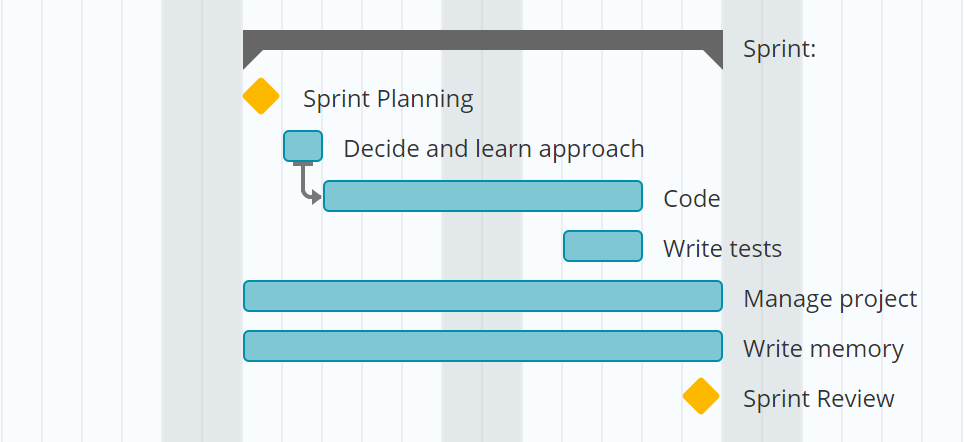
\includegraphics[width=10cm]{media/diagrams/gantt-sprint.png}
\end{center}
\caption[Sprint Gantt diagram]{Sprint Gantt diagram}
\label{fig:sprint_gantt}
\end{figure}

\begin{table}[]
    \centering
    \begin{singlespace}
    
    \begin{tabular}{lr} 
    \toprule
    \textbf{Sprint} & \textbf{50h} \\
    \midrule
    \hspace{3mm}Decide and learn approach & 5h \\
    \hspace{3mm}Code & 20h \\
    \hspace{3mm}Write tests & 5h \\
    \hspace{3mm}Manage project & 5h \\
    \hspace{3mm}Write memory & 15h \\
    \bottomrule
    \end{tabular}
    \end{singlespace}
    
    \caption{Description of sprint tasks and estimations}
    \label{sprint-task-list}
\end{table}

\subsection{Description of tasks}
\label{sec:schedule-blocks}

The project is split up into 4 blocks. See table \ref{task-list}.

\begin{itemize}
    \item \textbf{Project Management}: Bound scope, create the planning, calculate the budget...
    \item \textbf{Development}: The app is developed.
    \item \textbf{Report}: Write the missing texts and review the entire document.
    \item \textbf{Defense}: Prepare the oral defense.
\end{itemize}

\begin{table}
    \centering
    \begin{singlespace}
    \begin{tabular}{lr} 
    \toprule
    \textbf{TASK} & \textbf{TIME} \\
    \midrule
    \textbf{Project Management} & \textbf{100h} \\
    \midrule
    \hspace{3mm}Document format & 10h \\
    \hspace{3mm}Write Context & 10h \\
    \hspace{3mm}Write Justification & 10h \\
    \hspace{3mm}Write Scope & 10h \\
    \hspace{3mm}Write Workflow & 10h \\
    \hspace{3mm}Write Schedule & 10h \\
    \hspace{3mm}Write Budget & 10h \\
    \hspace{3mm}Write Sustainability & 10h \\
    \hspace{3mm}Review and finish document & 20h \\
    \midrule
    \textbf{Development} & \textbf{275h} \\
    \midrule
    \hspace{3mm}Sprint 1 & 50h \\
    \hspace{3mm}Sprint 2 & 50h \\
    \hspace{3mm}Sprint 3 & 50h \\
    \hspace{3mm}Sprint 4 & 50h \\
    \hspace{3mm}Sprint 5 & 50h \\
    \hspace{3mm}Sprint 6 & 25h \\
    \midrule
    \textbf{Report} & \textbf{50h} \\
    \midrule
    \hspace{3mm}Write report & 25h \\
    \hspace{3mm}Review report & 25h \\
    \midrule
    \textbf{Defense} & \textbf{50h} \\
    \midrule
    \hspace{3mm}Write script & 10h \\
    \hspace{3mm}Make slides & 10h \\
    \hspace{3mm}Design demo & 5h \\
    \hspace{3mm}Practice & 25h \\
    \midrule
    \textbf{TOTAL} & \textbf{475h} \\
    \bottomrule
    \end{tabular}
    \end{singlespace}
    
    \caption{Description of tasks and estimations}
    \label{task-list}
\end{table}

\newpage
\subsection{Gantt diagram}

\begin{figure}[ht!]
\begin{center}
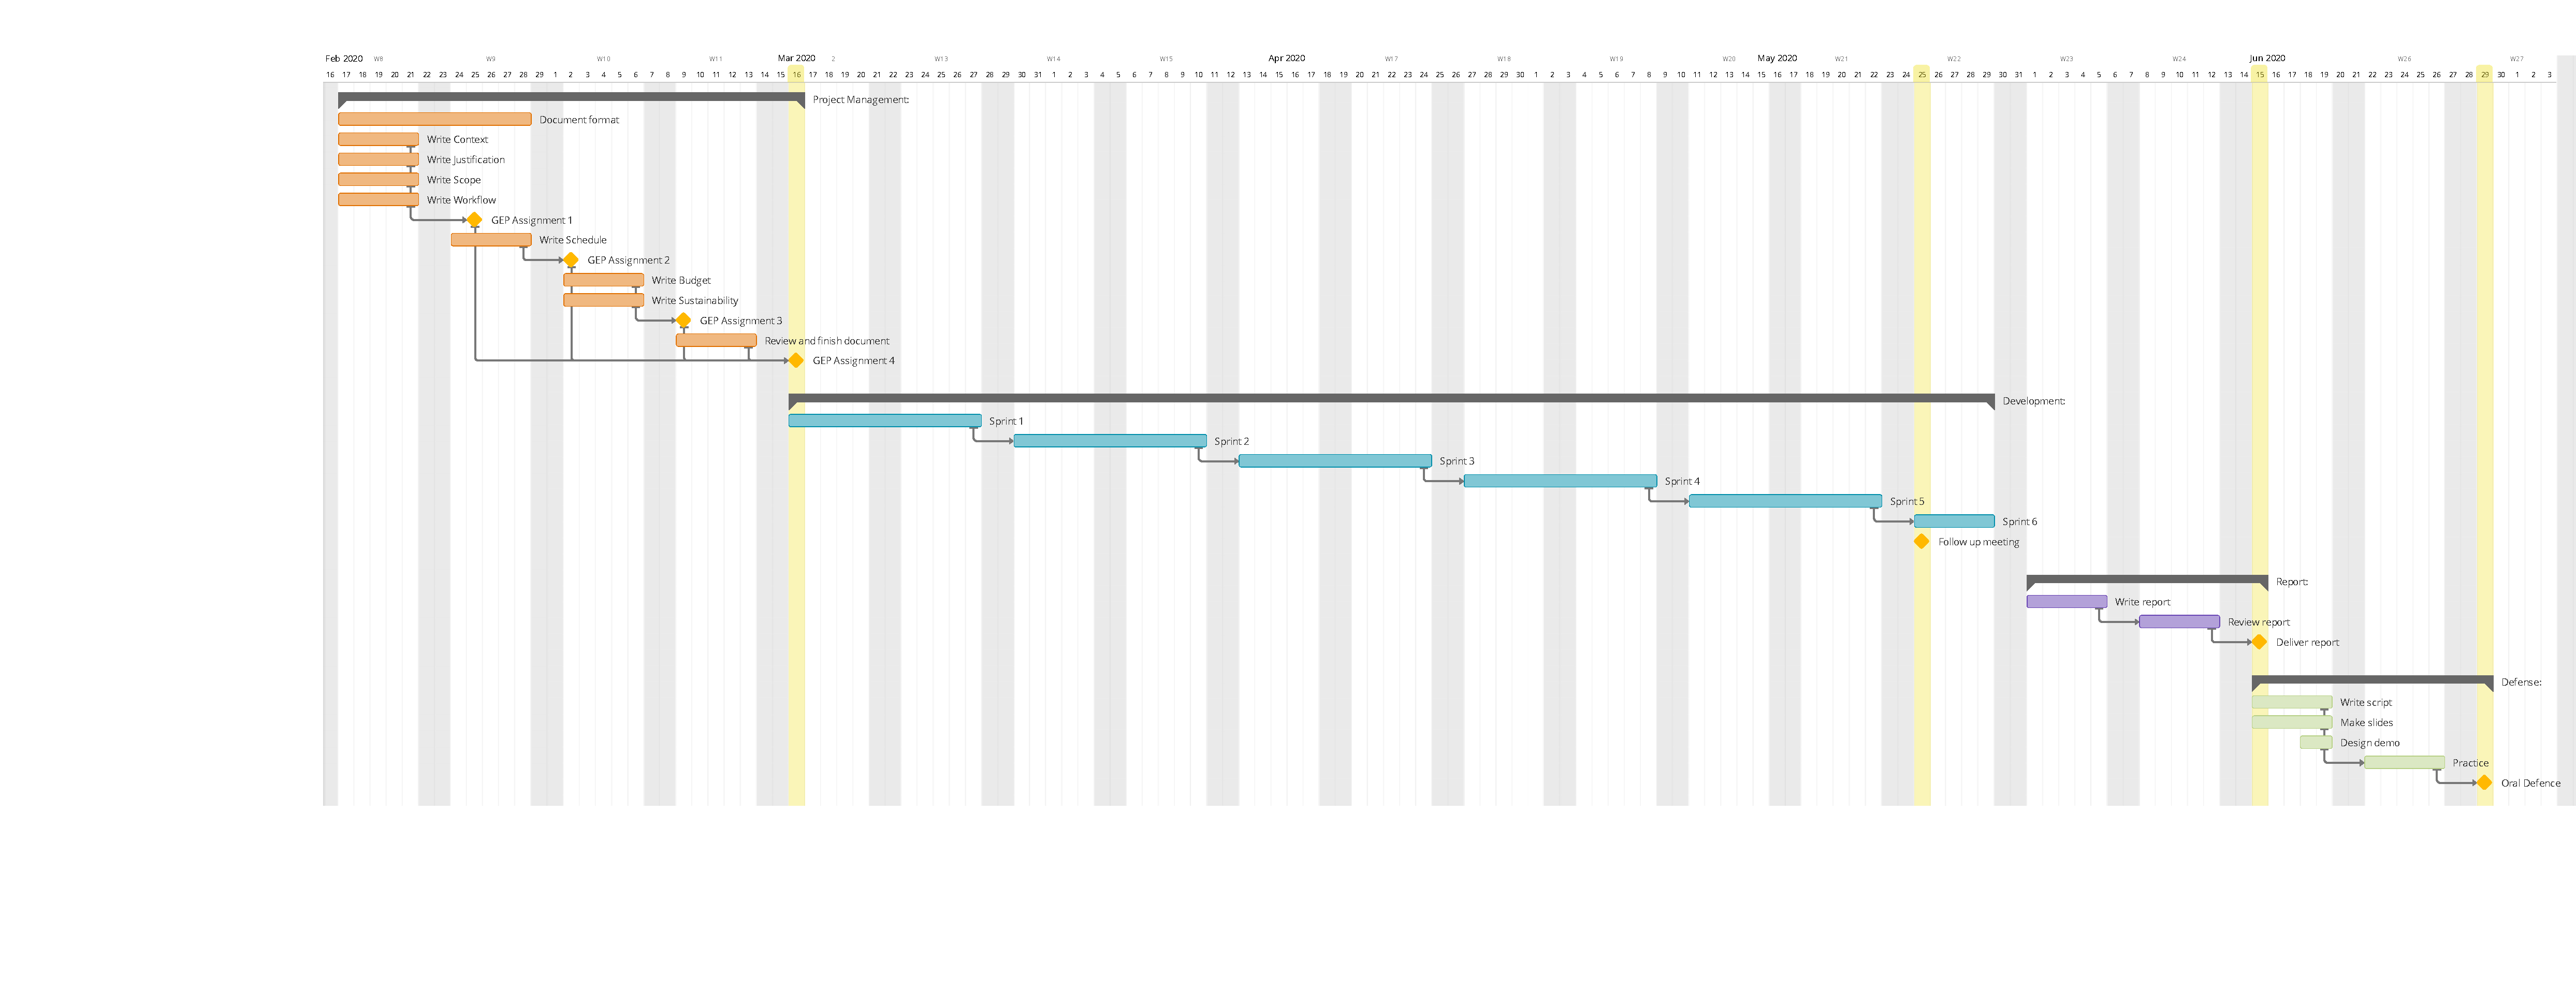
\includegraphics[width=\textheight-79pt,angle=90]{media/diagrams/gantt.pdf}
\end{center}
\caption[Gantt diagram]{Gantt diagram}
\label{gantt}
\end{figure}

\subsubsection{Dependencies}

\begin{itemize}
    \item \textbf{Project Management}: Each GEP assignment doesn't require the previous ones, except the last one that requires all of them.
    \item \textbf{Development}: Each sprint starts when the previous one finishes, they can't overlap and the order doesn't matter.
    \item \textbf{Memory}: To start reviewing the memory, it must be finished.
    \item \textbf{Defense}: To start practicing the oral defense, it must be finished.
\end{itemize}

\subsection{Required resources}

All this project is thought to be developed by one person, me. The only required material resource is a computer.

\subsection{Risk management: alternative plans and obstacles}

The main risks are explained in section \ref{sec:risks}. These are the mitigation of the problems:

% In the case of not having enough time to finish, a seventh sprint would be added, delaying the report and defense 2 weeks. This would give a fantastic 50 extra hours. In the follow-up meeting, it will be decided if this sprint is added.

% In the opposite case, having too much time left, more tasks would be added to the backlog.

\begin{table}[ht!]
    \centering
    \begin{singlespace}

    \begin{tabularx}{\textwidth}{lllX} 
    \toprule
    \textbf{Risk} & \textbf{Probability} & \textbf{Impact} & \textbf{Mitigations} \\
    \midrule
    \hspace{3mm}No decent free option. & High & Medium & A. Check is the free tier is enough.\newline B. Find alternatives.\newline C. Pay if it's really important.\newline \\
    \hspace{3mm}Not enough time. & Medium & High & A. Quit other activities.\newline B. Reduce scope.\newline C. Ask additional enrolment.\newline \\
    \hspace{3mm}Too much to learn. & Medium & Medium & A. Do a workaround.\newline B. Use something else.\newline C. Skip the task. \\
    \bottomrule
    \end{tabularx}
    
    \end{singlespace}
    \caption{Risks and mitigations}
    \label{risk-list}
\end{table}

\subsection{Changes in the schedule}

The main changes in the planning (chapter \ref{chap:schedule}) have been in the Development phase. The other blocks (section \ref{sec:schedule-blocks}) didn't have significant changes.

I followed the Kanban methodology, but I didn't do the formal sprint reviews I planned to. So because there were no sprint reviews there weren't sprints neither. 

Instead of grouping the tasks in sprints, the project evolved into a more fluid methodology where I was completing tasks faster than I expected in general.

Not framing the tasks inside sprints had a positive impact on my performance because when a task was getting too complicated I could leave it aside, do other tasks and come back to it once some time passed. When retrying a task I had a fresher perspective and better ideas because I had time to come up with alternative solutions.

Another deviation is that I didn't write the memory while developing, so the last sprint (the 6th) was devoted to writing the follow-up report.

The follow-up meeting was scheduled on the Friday 29th of May.

The memory delivery date was scheduled on Thursday 25th of June, and the defense date on Thursday 2nd of July.

The writing time of the memory was stretched until the deadline, and the presentation was done in one week.

\newpage
\subsubsection{Updated Gantt diagram}

\begin{figure}[ht!]
    \center
    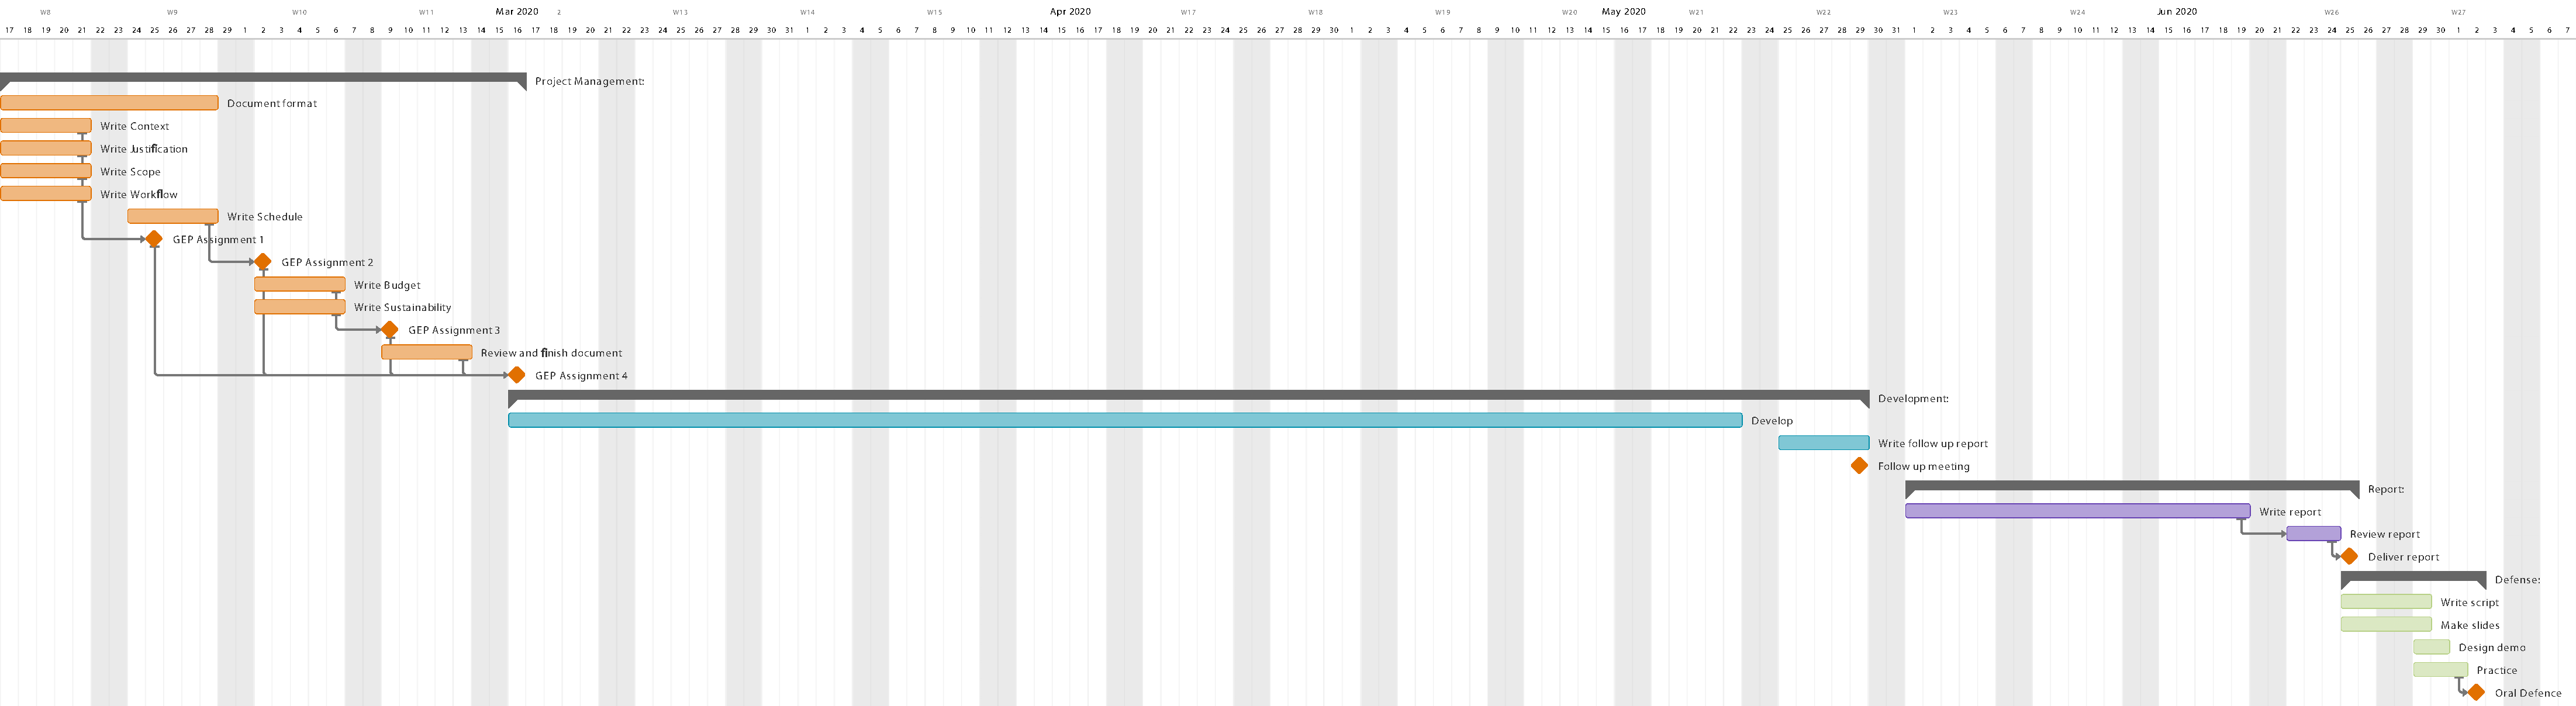
\includegraphics[width=\textheight-79pt,angle=90]{media/diagrams/gantt2.pdf}
    \caption{Updated Gantt diagram}
    \label{updated-gantt}
\end{figure}
